\begin{frame}{Separation of $d(K^-, n)"\pi^{\mp}\Sigma^{\pm}"$}
  \label{page:tempFit}
  
  \begin{tabular}{cc}
    \begin{minipage}{0.5\hsize}
      \begin{figure}
        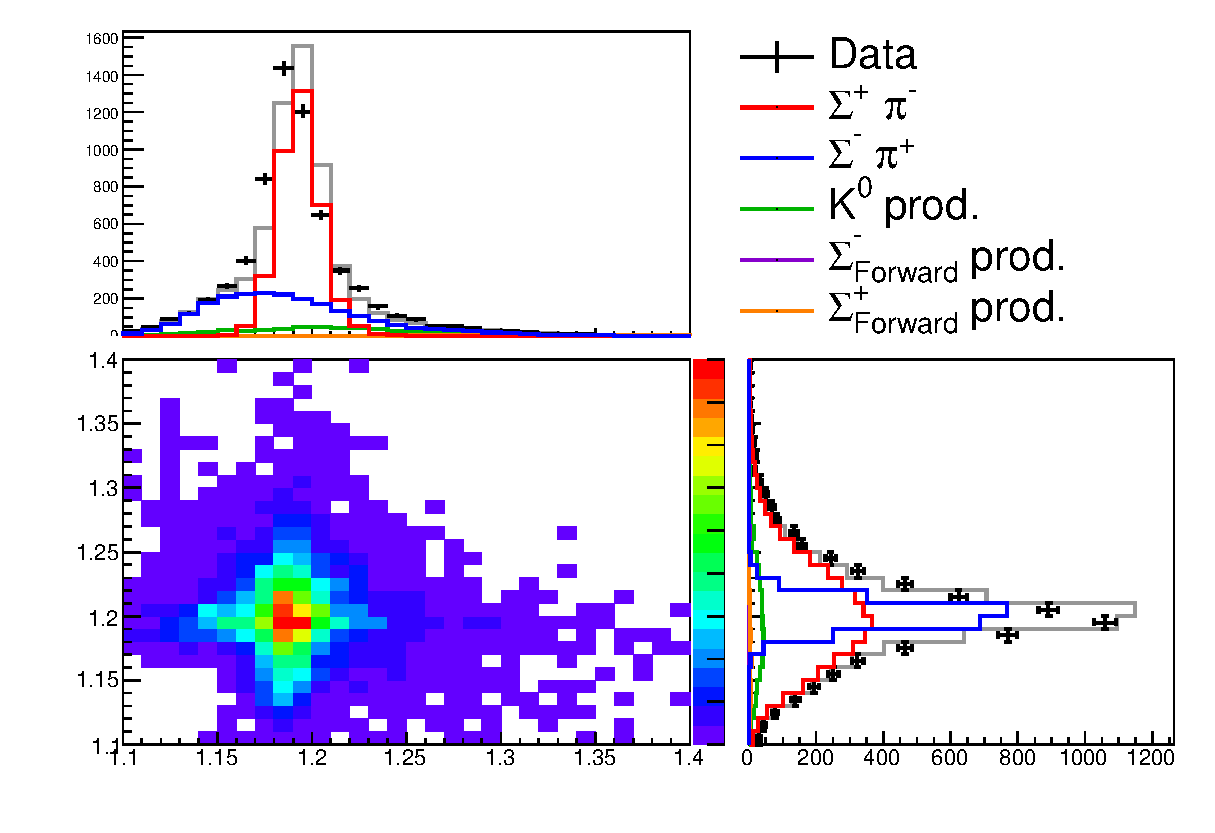
\includegraphics[width=4.5cm]{../pic/Run78/KN_ana_NC170_2sigma/KNpim_KNpip_MM.eps}
      \end{figure}
      \vspace{-5mm}
      \centering
      \tiny
      The figure shows summed all bin of $d(K^-, n)"X"$.
      
    \end{minipage}
    
    \begin{minipage}{0.5\hsize}
      \begin{itemize}
      \item $d(K^-, n)"\pi^-\Sigma^+"$\\
        {
          \scriptsize
          In $d(K^-, n \pi^-)"X"$, $\Sigma^+$ peak is seen like up figure\\
          In $d(K^-, n \pi^+)"X"$, widly distribution like side figure\\
        }
      \item $d(K^-, n)"\pi^+\Sigma^-"$\\
        { \scriptsize
          Opposite chage of $d(K^-, n)"\pi^-\Sigma^+"$。\\
        }
      \end{itemize}
      \centering
      \tiny
      bin-by-bin result in p.\pageref{page:fitKNpi},\pageref{page:fitKNpi2}
    \end{minipage}
  \end{tabular}

  \tminipageTwo{
    \begin{figure}
      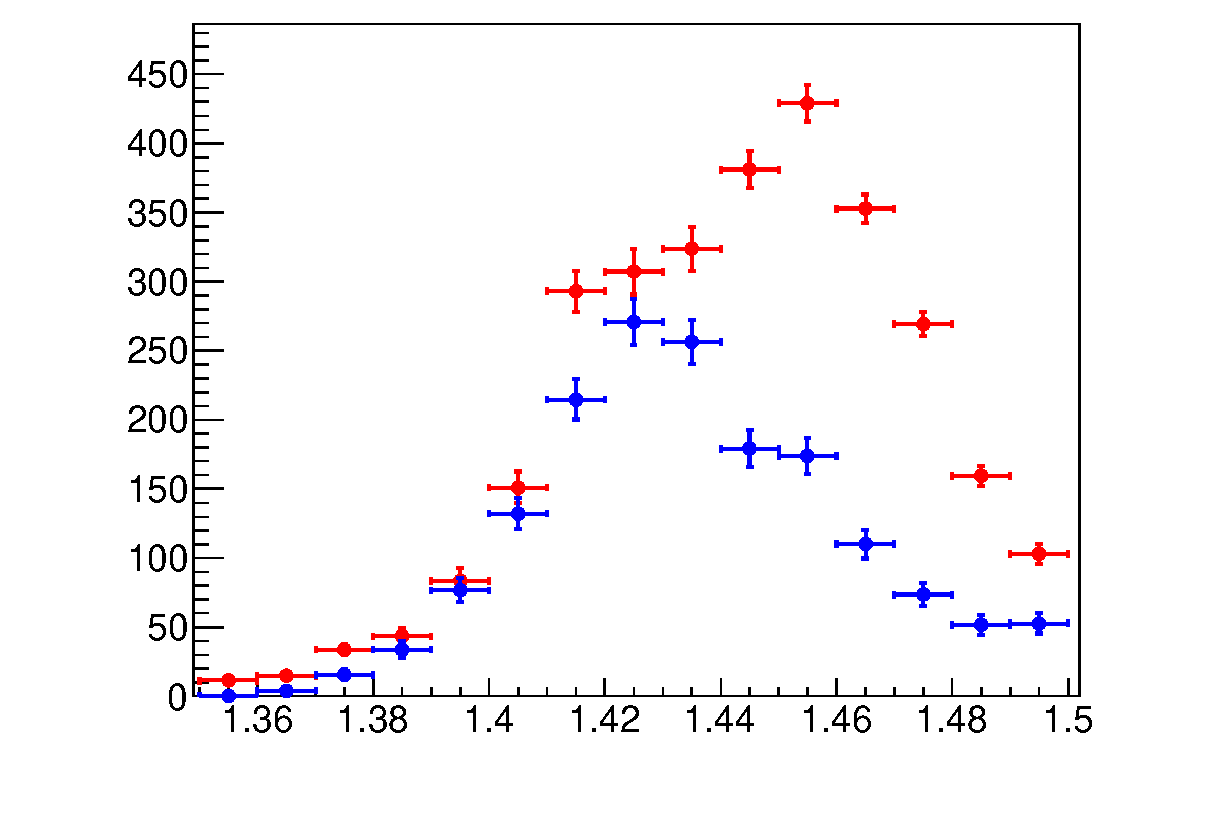
\includegraphics[width=4.5cm]{../pic/Run78/KN_ana_NC170_2sigma/piS_num.eps}
    \end{figure}
    \vspace{-5mm}
    \centering
    \tiny
    Separated $d(K^-, n)"\pi^{\mp}\Sigma^{\pm}"$ counts    
  }{
    \begin{figure}
      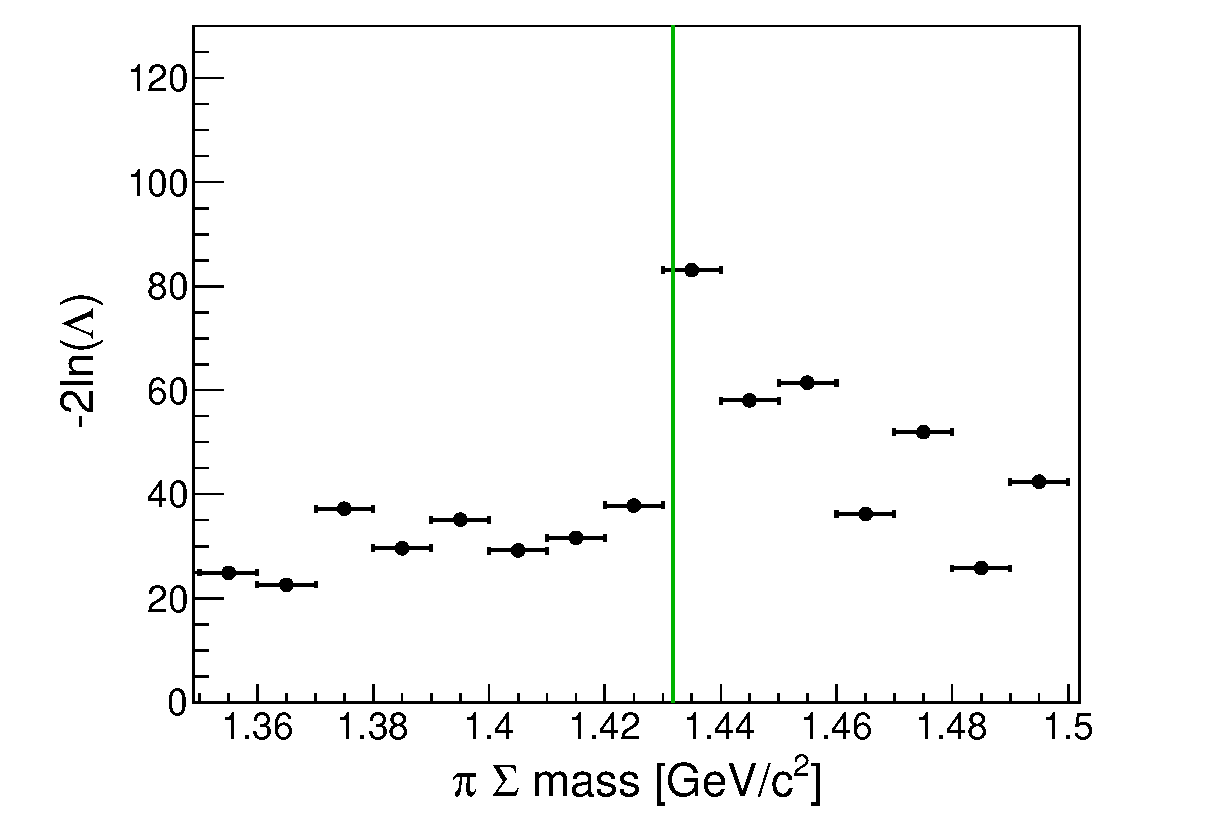
\includegraphics[width=4.5cm]{../pic/Run78/KN_ana_NC170_2sigma/Chi2.eps}
    \end{figure}
    \vspace{-5mm}
    \centering
    \tiny
    Loglikelihood of $d(K^-, n \pi^{\mp})"\Sigma^{\pm}"$ fitting
  }
\end{frame}
